\begin{frame}{Negative Binomial Generalized Linear Model}
  Let \(X_{ij}\) represent the UMI counts for the gene \(i\) in the cell \(j\)
  \begin{align}
    X_{ij} &\sim NB(\mu_{ij}, \phi_i) \\
    \mu_{ij}  &= S_j * \lambda_{ij} \\
    \log(\lambda_{ij})  &= \sum_r d_{jr} \beta_{ir} \\
    \phi_{i} &\sim Gamma(\alpha_0, \beta_0) 
  \end{align}
  \begin{equation*}
    \resizebox{0.6\hsize}{!}{$%
    \bm{\beta_r} \sim {\cal N}\left(\bm{0}, 
    \begin{bmatrix}
      \sigma_0^2  &     & & & &\\
      &   \myemph{\sigma_{ind}^2} & & & &\\
      &    &     \ddots &      & & \\
      &    &     & \myemph{\sigma_{ind}^2}  & & \\
      &    &     &  &   \mywarn{\sigma_{cond}^2} &  \\
      &    &     &   &    &  \mywarn{\sigma_{cond}^2} 
      \end{bmatrix}
    \right)
    $%
    }%
  \end{equation*}
  \begin{equation*}
    \mathbf{d_j} = \left(1, \overbrace{(0, \myemph{1}, \dots, 0, 0)}, \underbrace{(\mywarn{1}, 0)}\right)
  \end{equation*}

\end{frame}

\begin{frame}
  \begin{figure}
    \centering
    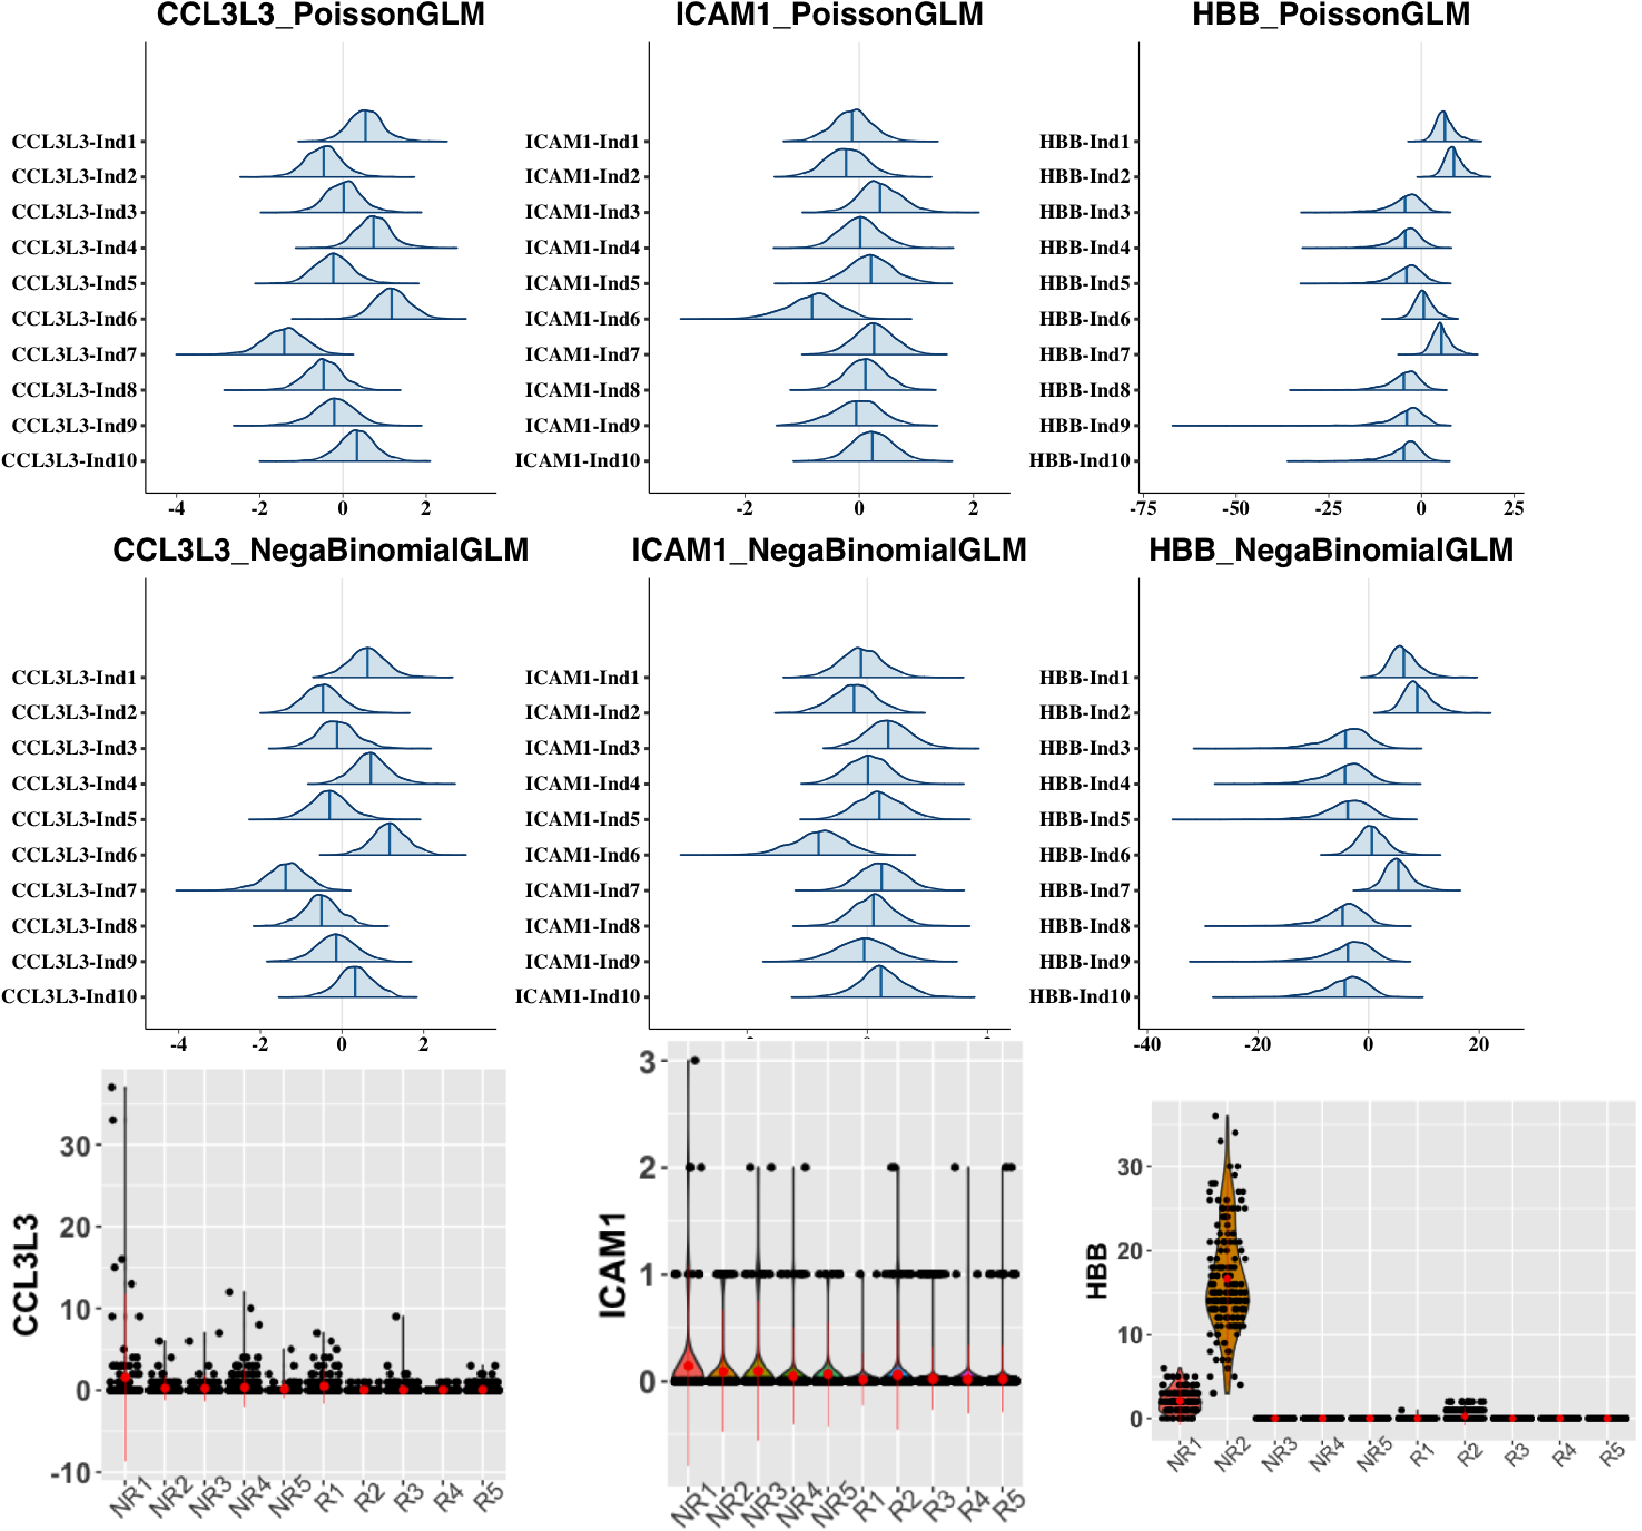
\includegraphics[height = \textheight]{poi_nb_pbmc_inds}
  \end{figure}
\end{frame}

\begin{frame}
  \begin{figure}
    \centering
    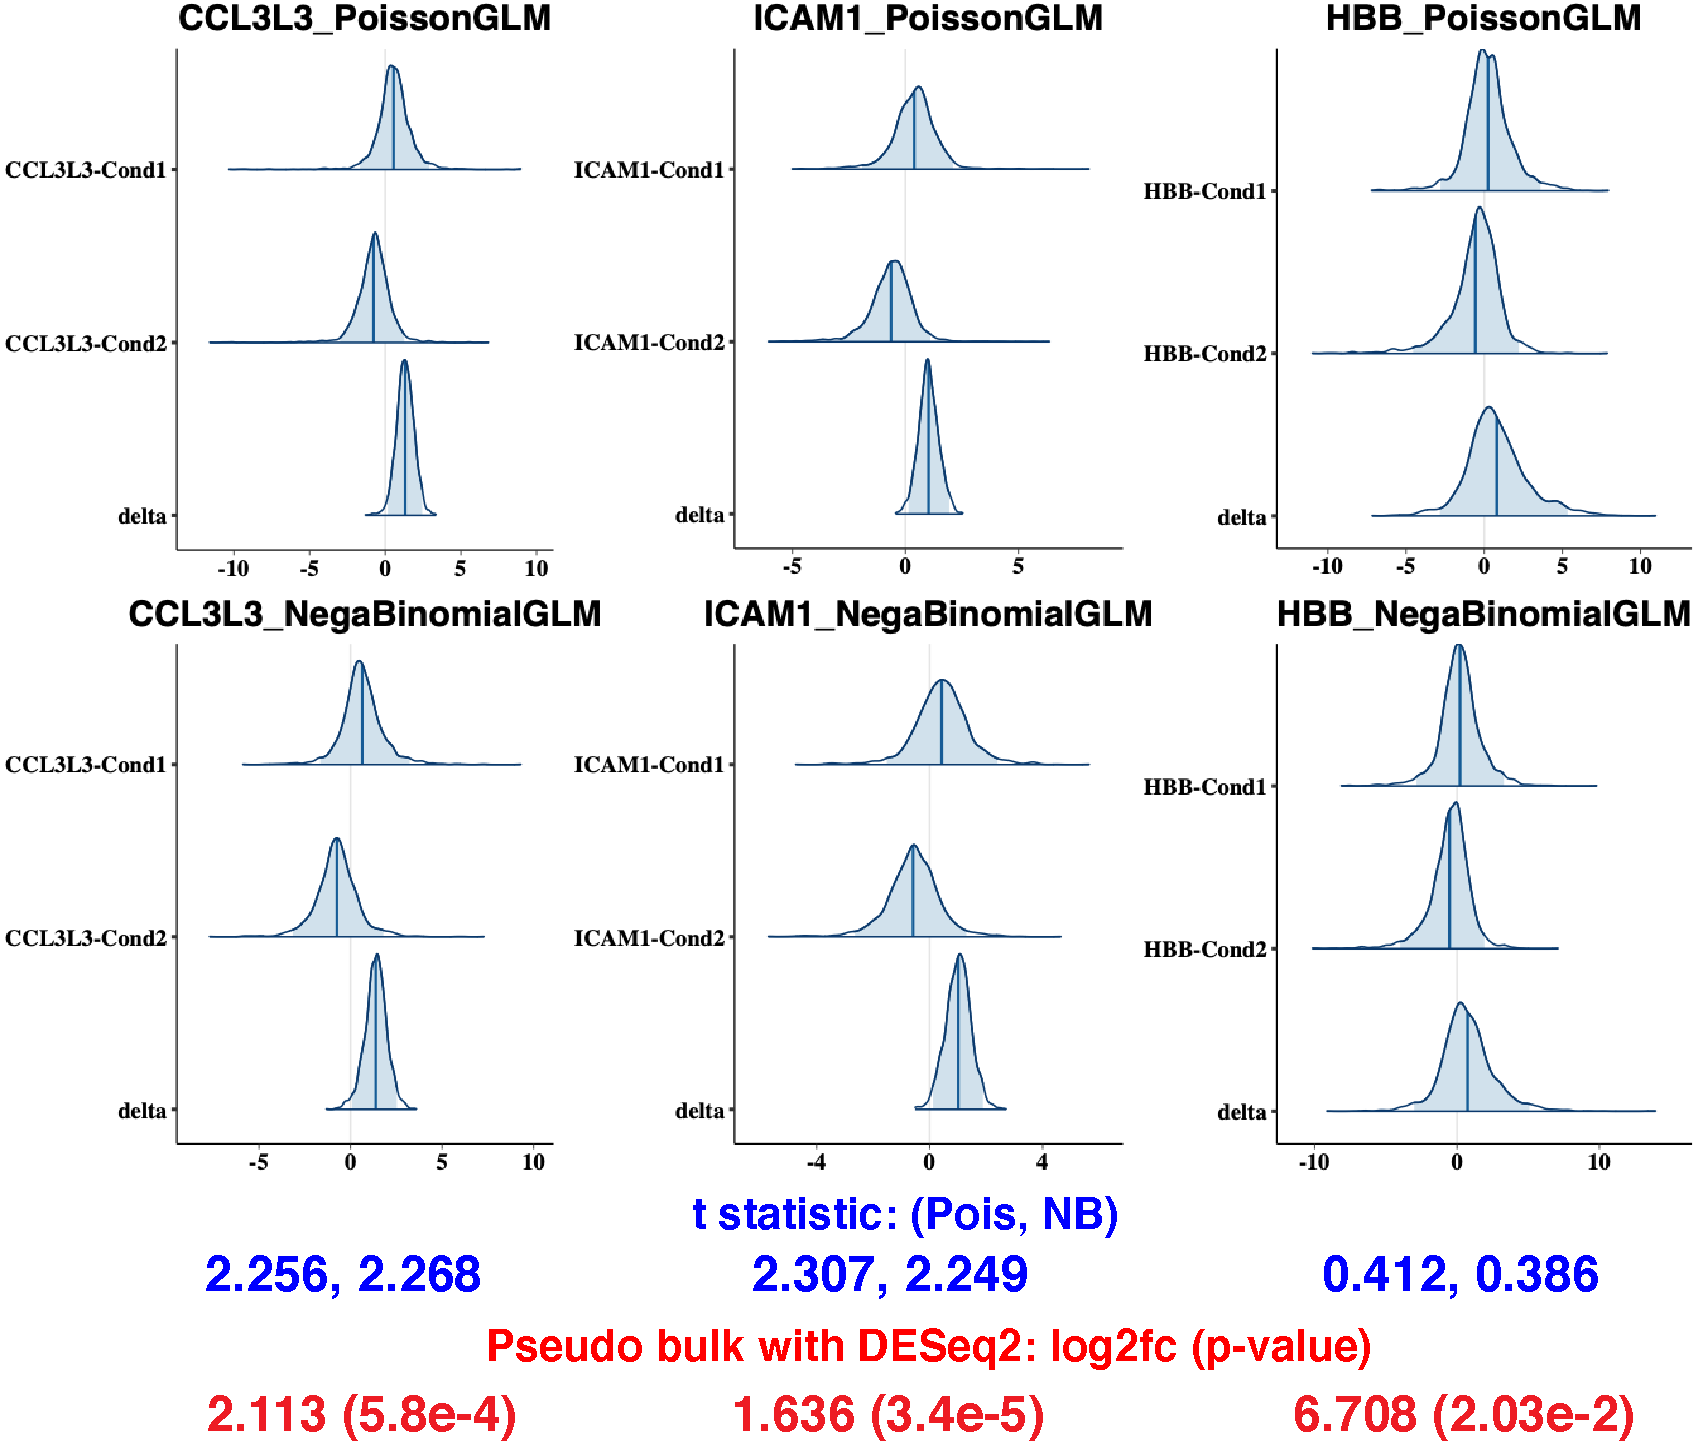
\includegraphics[height = \textheight]{poi_nb_pbmc_conds_with_scores}
  \end{figure}
\end{frame}
